\documentclass[8pt,a4paper,compress]{beamer}

\usepackage{/home/siyer/lib/slides}

\title{Shortest Paths}
\date{}
\begin{document}
\begin{frame}
\vfill
\titlepage
\end{frame}

\begin{frame}
\frametitle{Outline}
\tableofcontents
\end{frame}

\section{Shortest Paths}
\begin{frame}[fragile]
\begin{itemize}
\item a shortest path from vertex $s$ to vertex $t$ in an edge-weighted digraph is a directed path from $s$ to $t$ with the property that no other such path has a lower weight

\begin{center}
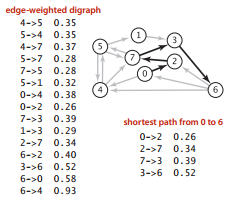
\includegraphics[scale=0.4]{./figures/sp1.png}

\smallskip

\small an edge-weighted digraph and a shortest path
\end{center}

\item variants: single source, single sink, source-sink, all pairs

\item typical shortest-paths applications
\begin{center}
\begin{tabular}{ccc}
\textbf{application} & \textbf{vertex} & \textbf{edge} \\ \hline \\
map & intersection & road \\
network & router & connection \\
schedule & job & precedence constraint \\
arbitrage & currency & exchange rate
\end{tabular}
\end{center}
\end{itemize}
\end{frame}

\section{Edge-Weighted Digraph API}
\begin{frame}[fragile]
\begin{itemize}
\item weighted directed edge data type: API and implementation
\begin{lstlisting}[language={},mathescape]
public class DirectedEdge

    DirectedEdge(int v, int w, double weight) // create a directed weighted 
                                              // edge $v$-$w$
    int from()      // vertex this edge points from
    int to()        // vertex this edge points to
    double weight() // weight of this edge
\end{lstlisting}

\begin{lstlisting}[language=Java]
public class DirectedEdge { 
    private final int v;
    private final int w;
    private final double weight;
    
    public DirectedEdge(int v, int w, double weight) {
        if (v < 0 || w < 0) { throw new IndexOutOfBoundsException(); }
        if (Double.isNaN(weight)) { throw new IllegalArgumentException(); }
        this.v = v;
        this.w = w;
        this.weight = weight;
    }

    public int from() { return v; }

    public int to() { return w; }

    public double weight() { return weight; }
    ...
}
\end{lstlisting}
\end{itemize}
\end{frame}

\begin{frame}[fragile]
\begin{itemize}
\item edge-weighted digraph (API)
\begin{lstlisting}[language={},mathescape]
public class EdgeWeightedDiGraph

    EdgeWeightedDigraph(int V)   // edge-weighted digraph with $V$ vertices
    EdgeWeightedDigraph(In in)   // edge-weighted digraph from input stream
    void addEdge(DirectedEdge e) // add weighted directed edge $e$
    Iterable<DirectedEdge> adj(int v) // edges pointing from $v$
    int V()                           // number of vertices
    int E()                           // number of edges
\end{lstlisting}
\end{itemize}
\end{frame}

\begin{frame}[fragile]
\begin{itemize}
\item edge-weighted digraph: implementation
\begin{lstlisting}[language=Java]
public class EdgeWeightedDigraph {
    private final int V;
    private int E;
    private LinkedBag<DirectedEdge>[] adj;
    
    public EdgeWeightedDigraph(int V) {
        if (V < 0) { throw new IllegalArgumentException(); }
        this.V = V;
        this.E = 0;
        adj = (LinkedBag<DirectedEdge>[]) new LinkedBag[V];
        for (int v = 0; v < V; v++) {
            adj[v] = new LinkedBag<DirectedEdge>();
        }
    }

    public EdgeWeightedDigraph(In in) {
        this(in.readInt());
        int E = in.readInt();
        if (E < 0) { throw new IllegalArgumentException(); }
        for (int i = 0; i < E; i++) {
            int v = in.readInt();
            int w = in.readInt();
            double weight = in.readDouble();
            addEdge(new DirectedEdge(v, w, weight));
        }
    }
    
    public int V() { return V; }

    public int E() { return E; }
    ...
}
\end{lstlisting}
\end{itemize}
\end{frame}

\begin{frame}[fragile]
\begin{itemize}
\item edge-weighted digraph: implementation (contd.)
\begin{lstlisting}[language=Java]
public class EdgeWeightedDigraph {
    ...
    public void addEdge(DirectedEdge e) {
        int v = e.from();
        int w = e.to();
        validateVertex(v);
        validateVertex(w);
        adj[v].add(e);
        E++;
    }

    public Iterable<DirectedEdge> adj(int v) {
        validateVertex(v);
        return adj[v];
    }

    public Iterable<DirectedEdge> edges() {
        LinkedBag<DirectedEdge> list = new LinkedBag<DirectedEdge>();
        for (int v = 0; v < V; v++) {
            for (DirectedEdge e : adj(v)) {
                list.add(e);
            }
        }
        return list;
    } 
    ...
}
\end{lstlisting}
\end{itemize}
\end{frame}

\section{Shortest Path API}
\begin{frame}[fragile]
\begin{itemize}
\item single-source shortest paths API
\begin{lstlisting}[language={},mathescape]
public class SP
    
    SP(EdgeWeightedDigraph G, int s) // constructor
    double distTo(int v)             // distance from $s$ to $v$, $\infty$ if no path
    boolean hasPathTo(int v)             // path from $s$ to $v$?
    Iterable<DirectedEdge> pathTo(int v) // path from $s$ to $v$, null if none
\end{lstlisting}

\item SP test client
\begin{lstlisting}[language=Java]
public class DijkstraSP {
    ...
    public static void main(String[] args) {
       In in = new In(args[0]);
        EdgeWeightedDigraph G = new EdgeWeightedDigraph(in);
        int s = Integer.parseInt(args[1]);
        DijkstraSP sp = new DijkstraSP(G, s);
        for (int t = 0; t < G.V(); t++) {
            if (sp.hasPathTo(t)) {
                StdOut.printf("%d to %d (%.2f)  ", s, t, sp.distTo(t));
                if (sp.hasPathTo(t)) {
                    for (DirectedEdge e : sp.pathTo(t)) {
                        StdOut.print(e + "   ");
                    }
                }
                StdOut.println();
            }
            else {
                StdOut.printf("%d to %d         no path\n", s, t);
            }
        }
    }
    ...
}
\end{lstlisting}
\end{itemize}
\end{frame}

\begin{frame}[fragile]
\begin{itemize}
\item SP test client (contd.)
\begin{lstlisting}[language={}]
$ java DijkstraSP tinyEWD.txt 0
0 to 0 (0.00):
0 to 1 (1.05): 0->4 0.38 4->5 0.35 5->1 0.32
0 to 2 (0.26): 0->2 0.26
0 to 3 (0.99): 0->2 0.26 2->7 0.34 7->3 0.39
0 to 4 (0.38): 0->4 0.38
0 to 5 (0.73): 0->4 0.38 4->5 0.35
0 to 6 (1.51): 0->2 0.26 2->7 0.34 7->3 0.39 3->6 0.52
0 to 7 (0.60): 0->2 0.26 2->7 0.34
\end{lstlisting}

\item a shortest-paths tree solution (SPT) always exists

\item data structures: can represent the SPT with two vertex-indexed arrays
\begin{itemize}
\item \lstinline{distTo[v]} is length of shortest path from $s$ to $v$

\item \lstinline{edgeTo[v]} is last edge on shortest path from $s$ to $v$
\end{itemize}

\begin{center}
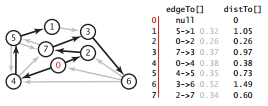
\includegraphics[scale=0.4]{./figures/sp2.png}

\smallskip

\small shortest-paths data structures
\end{center}
\end{itemize}
\end{frame}

\begin{frame}[fragile]
\begin{itemize}
\item edge relaxation: relax edge $e = v\to w$
\begin{itemize}
\item \lstinline{distTo[v]} is length of shortest known path from $s$ to $v$

\item \lstinline{distTo[w]} is length of shortest known path from $s$ to $w$

\item \lstinline{edgeTo[w]} is last edge on shortest known path from $s$ to $w$

\item if $e = v\to w$ gives shorter path to $w$ through $v$, update both \lstinline{distTo[w]} and \lstinline{edgeTo[w]}
\end{itemize}

\begin{lstlisting}[language=Java]
private void relax(DirectedEdge e) {
    int v = e.from(), w = e.to();
    if (distTo[w] > distTo[v] + e.weight()) {
        distTo[w] = distTo[v] + e.weight();
        edgeTo[w] = e;
    }
}
\end{lstlisting}

\begin{center}
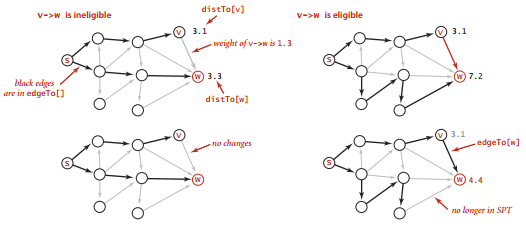
\includegraphics[scale=0.4]{./figures/sp3.png}

\smallskip

\small edge relaxation (two cases)
\end{center}
\end{itemize}
\end{frame}

\section{Dijkstra's Algorithm}
\begin{frame}[fragile]
\begin{itemize}
\item Dijkstra's algorithm computes a SPT in any edge-weighted
digraph with nonnegative weights

\item procedure
\begin{itemize}
\item consider vertices in increasing order of distance from $s$ (non-tree vertex with the lowest \lstinline{distTo[]} value)

\item add vertex to tree and relax all edges pointing from that vertex
\end{itemize}

\item implementation
\begin{lstlisting}[language=Java]
public class DijkstraSP {
    private double[] distTo; 
    private DirectedEdge[] edgeTo; 
    private IndexMinPQ<Double> pq; 
    
    public DijkstraSP(EdgeWeightedDigraph G, int s) {
        for (DirectedEdge e : G.edges()) {
            if (e.weight() < 0) { throw new IllegalArgumentException(...); }
        }
        distTo = new double[G.V()];
        edgeTo = new DirectedEdge[G.V()];
        for (int v = 0; v < G.V(); v++) { 
            distTo[v] = Double.POSITIVE_INFINITY; 
        }
        distTo[s] = 0.0;
        pq = new IndexMinPQ<Double>(G.V());
        pq.insert(s, distTo[s]);
        while (!pq.isEmpty()) {
            int v = pq.delMin();
            for (DirectedEdge e : G.adj(v)) { relax(e); }
        }
    }    
    ...
}
\end{lstlisting}
\end{itemize}
\end{frame}

\begin{frame}[fragile]
\begin{minipage}{220pt}
\begin{itemize}
\item implementation (contd.)
\begin{lstlisting}[language=Java]
public class DijkstraSP {
    ...
    public double distTo(int v) { 
        return distTo[v]; 
    }

    public boolean hasPathTo(int v) { 
        return distTo[v] < Double.POSITIVE_INFINITY; 
    }
    
    public Iterable<DirectedEdge> pathTo(int v) {
        if (!hasPathTo(v)) { return null; }
        LinkedStack<DirectedEdge> path = 
            new LinkedStack<DirectedEdge>();
        for (DirectedEdge e = edgeTo[v]; e != null; 
            e = edgeTo[e.from()]) {
            path.push(e);
        }
        return path;
    }
    ...
}
\end{lstlisting}

\item Dijkstra's algorithm using a binary heap based priority queue computes a SPT in an edge-weighted digraph in time proportional to $E\log V$ in the worst case
\end{itemize}
\end{minipage}%
\begin{minipage}{80pt}
\begin{center}
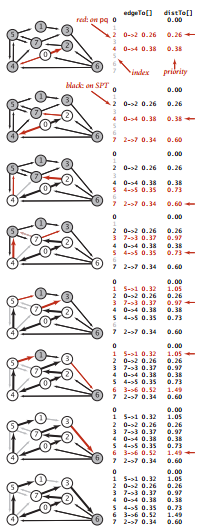
\includegraphics[scale=0.42]{./figures/sp4.png}

\smallskip

\small trace of Dijkstra's algorithm
\end{center}
\end{minipage}
\end{frame}

\section{Edge-Weighted DAGs}
\begin{frame}[fragile]
\begin{itemize}
\item it is easier to find shortest paths in an edge-weighted DAG than in a general digraph
\begin{itemize}
\item consider vertices in topological order

\item relax all edges pointing from that vertex
\end{itemize}

\item topological sort algorithm computes SPT in any edge-weighted DAG in time proportional to $E + V$

\item implementation
\begin{lstlisting}[language=Java]
public class AcyclicSP {
    private double[] distTo; 
    private DirectedEdge[] edgeTo; 
    
    public AcyclicSP(EdgeWeightedDigraph G, int s) {
        distTo = new double[G.V()];
        edgeTo = new DirectedEdge[G.V()];
        for (int v = 0; v < G.V(); v++) {
            distTo[v] = Double.POSITIVE_INFINITY;
        }
        distTo[s] = 0.0;
        Topological topological = new Topological(G);
        if (!topological.hasOrder()) { 
            throw new IllegalArgumentException(); 
        }
        for (int v : topological.order()) {
            for (DirectedEdge e : G.adj(v)) { relax(e); }
        }
    }
    ...
}
\end{lstlisting}
\end{itemize}
\end{frame}

\begin{frame}[fragile]
\begin{minipage}{220pt}
\begin{itemize}
\item implementation (contd.)
\begin{lstlisting}[language=Java]
public class AcyclicSP {
    ...
    public double distTo(int v) { 
        return distTo[v]; 
    }

    public boolean hasPathTo(int v) { 
        return distTo[v] < Double.POSITIVE_INFINITY; 
    }
    
    public Iterable<DirectedEdge> pathTo(int v) {
        if (!hasPathTo(v)) { return null; }
        LinkedStack<DirectedEdge> path = 
            new LinkedStack<DirectedEdge>();
        for (DirectedEdge e = edgeTo[v]; e != null; 
            e = edgeTo[e.from()]) {
            path.push(e);
        }
        return path;
    }
    ...
}
\end{lstlisting}
\end{itemize}
\end{minipage}%
\begin{minipage}{80pt}
\begin{center}
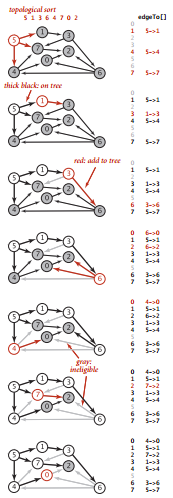
\includegraphics[scale=0.42]{./figures/sp5.png}

\smallskip

\small trace of shortest paths in edge-weighted DAG
\end{center}
\end{minipage}
\end{frame}

\begin{frame}[fragile]
\begin{itemize}
\item applications
\begin{itemize}
\item seam carving: resize an image without distortion for display on cell phones and web browser

\item longest paths in edge-weighted DAGs: formulate as a shortest paths problem in edge-weighted DAGs (topological sort algorithm works even with negative weights; see \lstinline{AcyclicLP})
\begin{itemize}
\item negate all weights

\item find shortest paths

\item negate weights in result
\end{itemize}

\item parallel job scheduling: given a set of jobs with durations and precedence
constraints, schedule the jobs (by finding a start time for each) so as to
achieve the minimum completion time, while respecting the constraints

\item critical path method: to solve a parallel job-scheduling problem, create edge-weighted DAG
\begin{itemize}
\item source and sink vertices
\item two vertices (begin and end) for each job
\item three edges for each job: begin to end (weighted by duration); source to begin (0 weight); and end to sink (0 weight)
\item one edge for each precedence constraint (0 weight)
\end{itemize}
and use longest path from the source to schedule each job (see \lstinline{CPM})
\end{itemize}
\end{itemize}
\end{frame}

\section{Negative Weights}
\begin{frame}[fragile]
\begin{itemize}
\item Dijkstra's algorithm does not work with negative edge weights

\item a negative cycle is a directed cycle whose sum of edge weights is
negative

\item to find a negative cycle, add two methods to the API for \lstinline{SP}
\begin{lstlisting}[language={},mathescape]
public class SP

    ...
    boolean hasNegativeCycle()              // is there a negative cycle?
    Iterable <DirectedEdge> negativeCycle() // negative cycle reachable 
                                            // from $s$
\end{lstlisting}

\item Bellman-Ford algorithm
\begin{itemize}
\item initialize \lstinline{distTo[]} to 0 for source vertex $s$ and $\infty$ for all other vertices $v$
\item relax each edge $V$ times
\end{itemize}

\item if there is a negative cycle, Bellman-Ford algorithm gets stuck in loop,
updating \lstinline{distTo[]} and \lstinline{edgeTo[]} entries of vertices in the cycle

\item if any vertex $v$ is updated in pass $v$, there exists a negative
cycle (and can trace back \lstinline{edgeTo[v]} entries to find it)
\end{itemize}
\end{frame}

\begin{frame}[fragile]
\begin{itemize}
\item Bellman-Ford algorithm: implementation
\begin{lstlisting}[language=Java]
public class BellmanFordSP {
    private double[] distTo; 
    private DirectedEdge[] edgeTo; 
    private boolean[] onQueue; 
    private LinkedQueue<Integer> queue; 
    private int cost;
    private Iterable<DirectedEdge> cycle;  
    
    public BellmanFordSP(EdgeWeightedDigraph G, int s) {
        distTo  = new double[G.V()];
        edgeTo  = new DirectedEdge[G.V()];
        onQueue = new boolean[G.V()];
        for (int v = 0; v < G.V(); v++) {
            distTo[v] = Double.POSITIVE_INFINITY;
        }
        distTo[s] = 0.0;
        queue = new LinkedQueue<Integer>();
        queue.enqueue(s);
        onQueue[s] = true;
        while (!queue.isEmpty() && !hasNegativeCycle()) {
            int v = queue.dequeue();
            onQueue[v] = false;
            relax(G, v);
        }
    }
    ...
}
\end{lstlisting}
\end{itemize}
\end{frame}

\begin{frame}[fragile]
\begin{itemize}
\item Bellman-Ford algorithm: implementation (contd.)
\begin{lstlisting}[language=Java]
public class BellmanFordSP {
    ...  
    private void relax(EdgeWeightedDigraph G, int v) {
        for (DirectedEdge e : G.adj(v)) {
            int w = e.to();
            if (distTo[w] > distTo[v] + e.weight()) {
                distTo[w] = distTo[v] + e.weight();
                edgeTo[w] = e;
                if (!onQueue[w]) {
                    queue.enqueue(w);
                    onQueue[w] = true;
                }
            }
            if (cost++ % G.V() == 0) { findNegativeCycle(); }
        }
    }
    
    public boolean hasNegativeCycle() { return cycle != null; }

    public Iterable<DirectedEdge> negativeCycle() { return cycle; }
    
    private void findNegativeCycle() {
        int V = edgeTo.length;
        EdgeWeightedDigraph spt = new EdgeWeightedDigraph(V);
        for (int v = 0; v < V; v++) {
            if (edgeTo[v] != null) { spt.addEdge(edgeTo[v]); }
        }
        EdgeWeightedDirectedCycle finder = 
            new EdgeWeightedDirectedCycle(spt);
        cycle = finder.cycle();
    }
    ...
}
\end{lstlisting}
\end{itemize}
\end{frame}

\begin{frame}[fragile]
\begin{itemize}
\item Bellman-Ford algorithm: implementation (contd.)
\begin{lstlisting}[language=Java]
public class BellmanFordSP {
    ...
    public double distTo(int v) {
        if (hasNegativeCycle()) { 
            throw new UnsupportedOperationException(); 
        }
        return distTo[v];
    }

    public boolean hasPathTo(int v) { 
        return distTo[v] < Double.POSITIVE_INFINITY; 
    }
    
    public Iterable<DirectedEdge> pathTo(int v) {
        if (hasNegativeCycle()) { 
            throw new UnsupportedOperationException(); 
        }
        if (!hasPathTo(v)) { return null; }
        LinkedStack<DirectedEdge> path = new LinkedStack<DirectedEdge>();
        for (DirectedEdge e = edgeTo[v]; e != null; e = edgeTo[e.from()]) {
            path.push(e);
        }
        return path;
    }
    ...
}
\end{lstlisting}

\item Bellman-Ford algorithm computes SPT in any edge-weighted digraph with no negative cycles in time proportional to $E \times V$
\end{itemize}
\end{frame}

\begin{frame}[fragile]
\begin{itemize}
\item Bellman-Ford algorithm: trace
\begin{center}

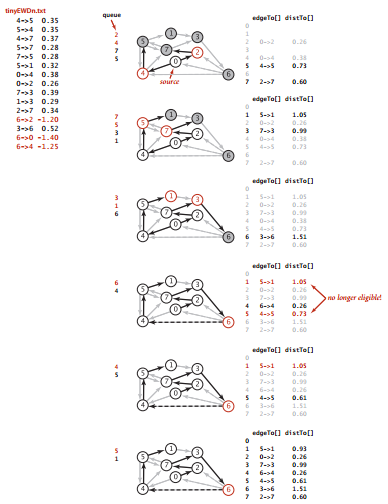
\includegraphics[scale=0.42]{./figures/sp6.png}

\smallskip

\small trace of Bellman-Ford algorithm (negative weights)
\end{center}
\end{itemize}
\end{frame}

\begin{frame}[fragile]
\begin{minipage}{200pt}
\begin{itemize}
\item negative cycle application: arbitrage detection (see \lstinline{Arbitrage})

\item currency exchange graph
\begin{itemize}
\item vertex = currency

\item edge = transaction, with weight equal to exchange rate

\item find a directed cycle whose product of edge weights is $> 1$
\end{itemize}

\item model as a negative cycle detection problem by taking logs
\begin{itemize}
\item let weight of edge $v \to w$ be $-\ln$(exchange rate from currency $v$ to $w$)

\item multiplication turns to addition; $> 1$ turns to $< 0$

\item find a directed cycle whose sum of edge weights is $< 0$ (negative cycle)
\end{itemize}
\end{itemize}
\end{minipage}%
\begin{minipage}{100pt}
\begin{center}
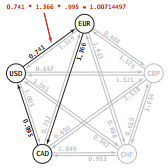
\includegraphics[scale=0.43]{./figures/sp7.png}

\smallskip

\small currency exchange graph

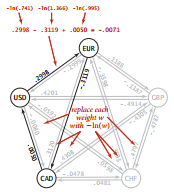
\includegraphics[scale=0.43]{./figures/sp8.png}

\smallskip

\small negative cycle represents an arbitrage opportunity
\end{center}
\end{minipage}
\end{frame}

\section{Summary}
\begin{frame}[fragile]
\begin{itemize}
\item nonnegative weights
\begin{itemize}
\item arises in many application
\item Dijkstra's algorithm is nearly linear-time
\end{itemize}

\item acyclic edge-weighted digraphs
\begin{itemize}
\item arise in some applications
\item topological sort algorithm is linear time
\item edge weights can be negative
\end{itemize}

\item negative weights and negative cycles
\begin{itemize}
\item arise in some applications
\item if no negative cycles, can find shortest paths via Bellman-Ford
\item if negative cycles, can find one via Bellman-Ford
\end{itemize}

\item shortest-paths is a broadly useful problem-solving model
\end{itemize}
\end{frame}
\end{document}
